%%%%%%%%%%%%%%%%%%%%%%%%%%%%%%%%%%%%%%%%%
%
% Funkcionalna verifikacija hardvera
% 
%%%%%%%%%%%%%%%%%%%%%%%%%%%%%%%%%%%%%%%%%

SystemVerilog jezik je nastao kao nadogradnja na Verilog 2001 jezik kako bi se
poboljšala produktivnost, čitljivost i ponovna upotreba koda.
Međutim, za razliku od Verilog-a i VHDL-a koji su jezici za opis hardvera i
neadekvatni za verifikaciju zbog svojih ograničenih osobina u pogledu raznih
programskih tehnika, SystemVerilog je prvi jezik u industriji za opis i
verifikaciju hardvera (engl. \emph{Hardware and Verification Language}, HDVL).
Kombinuje osobine VHDL i Verilog-a, sa osobinama C i C++ jezika. Neke od
karakteristika SystemVerilog-a su uvođenje objektno-orijentisanog mehanizma,
velika mogućnost randomizacije, podrška za funkcionalnu pokrivenost
(\emph{coverage}), ...\\

U ovoj vežbi su objašnjene osnove SystemVerilog jezika, dat je pregled osnovnih
pojmova, tipova podataka kao i poređenje sa već poznatim konstrukcijama iz VHDL
jezika.

%========================================================================================
% Section
%========================================================================================

\section{VHDL \(\rightarrow\) SystemVerilog}

U nastavku je dat pregled osnovnih pojmova u SystemVerilog-u i izvršeno
poređenje sa VHDL jezikom.\\

Kao što se vidi na primeru 4-bitnog brojača, iako implementiraju isti model, kod
pisan u VHDL-u (kod \ref{lst:VHDL_brojac}) i SystemVerilog-u (kod
\ref{lst:SV_brojac}) se dosta razlikuje.
Sintaksa SystemVerilog-a umnogome podseća na sintaksu C jezika, što daje velik
kontrast VHDL-u koji po sintaksi podseća više na Pascal ili Ada jezik.

\lstinputlisting[language=VHDL, caption=VHDL brojac, label=lst:VHDL_brojac]{code/v1_counter.vhd}
\lstinputlisting[caption=SystemVerilog brojac, label=lst:SV_brojac]{code/v1_counter.sv}

%----------------------------------------------------------------------------------------

\subsection{Modul}

\emph{Entity-architecture} par koji se koristi u VHDL-u je objedinjen je u
Verilog/SystemVerilog jeziku uvođenjem koncepta modula. Modul objedinjuje i
opis interfejsa i opis funkcionalnosti. Sintaksa modula prikazana je ispod:

\begin{lstlisting}
module module_name (port_list);
  input  [msb:lsb] input_port_list;
  output [msb:lsb] output_port_list;
  inout  [msb:lsb] inout_port_list;
  // ... statements ...
endmodule
\end{lstlisting}

Kao i u VHDL-u, portovi mogu biti ulazni, izlazni i ulazno-izlazni. Višebitni
portovi se opisuju navođenjem opsega bita u uglastim zagradama.

%----------------------------------------------------------------------------------------

\subsection{\emph{Continuous assignments}}

\emph{Concurrent assignments} u VHDL-u se obično nazivaju \emph{continuous
  assignments} u SystemVerilog-u. Sintaksa je sledeća:

\begin{lstlisting}
assign wire_variable = expression;
\end{lstlisting}

Kao i u VHDL-u, redosled ovih naredbi nije bitan.
Takođe, se može uslovno dodeljivati vrednost.

\begin{lstlisting}[language=VHDL]
data_o <= a when (sel = '1') else b;
\end{lstlisting}
\begin{lstlisting}
assign data_o = sel ? a : b;
\end{lstlisting}

Na ovom jednostavnom primeru uslovne dodele se vrlo lako lako uočava velika
sličnost sa C jezikom.

%----------------------------------------------------------------------------------------

\subsection{Proceduralni blokovi}

Procese u VHDL-u zamenjuju \emph{always} blokovi.
Postoje četiri vrste \emph{always} blokova.
\begin{itemize}
\item \emph{always}: generalna procedura. Najčešće se koristi u verifikaciji za
  generisanje takta.
  \begin{lstlisting}
always #10 clk =~clk;
\end{lstlisting}
\item \emph{always\(\_\)ff}: za modelovanje sekvencijalne logike. Moguće
  limitirati reakciju bloka na određenu ivicu koristeći ključne reči
  \emph{posedge} i \emph{negedge}, za rastuću i opadajuću ivicu, respektivno.
  \begin{lstlisting}
always_ff @(posedge clock iff reset == 0 or posedge reset) begin
  r1 <= reset ? 0 : r2 + 1;
  // ...
end
\end{lstlisting}
\item \emph{always\(\_\)comb}: za modelovanje kombinacione logike. U ovom bloku
  je lista osetljivosti implicitna i sadrži sve signale koji se koriste u bloku.
  \begin{lstlisting}
always_comb
  a = b & c;
\end{lstlisting}
\item \emph{always\(\_\)latch}: koristi se za modelovanje lečeva.
  \begin{lstlisting}
always_latch
  if (load) q <= d;
\end{lstlisting}
\end{itemize}

Pored \emph{always}, postoje još dve vrste proceduralnih blokova.
To su \emph{initial} i \emph{final} blokovi.
\emph{Initial} blokovi se izvršavaju samo jednom, na početku simulacije.
U VHDL-u bi to bio proces sa \emph{wait} naredbom na kraju.
Slično je i sa \emph{final} blokom koji se izvršava na kraju simulacije.

%----------------------------------------------------------------------------------------

\subsection{Kašnjenje}

\emph{Wait} naredba iz VHDL se može koristiti za razne vrste kašnjenja
(vremensko kašnjenje, čekanje na signal itd.).
U SystemVerilogu se kašnjenje moze podeliti na tri tipa:

\begin{itemize}
\item Vremensko kašnjenje:
  specificira se \(\#\) operatorom (npr. \(\#\)5ns – čeka 5 ns pre izvršavanja
  sledeće naredbe). Moguće jedinice su fs, ps, ns, us, ms, s.
\item Čekanje na događaj (engl. \emph{event}):
  specificira se sa @ (npr. @(clk) – blokira izvršavanje dok se ne desi promena
  na clk signalu). Korišćenje \emph{event}-ova će biti detaljno objašnjeno u
  vežbi o inter-proces komunikaciji.
\item Čekanje na uslov:
  specificira se sa \emph{wait} naredbom koja je ekvivalentna VHDL-ovoj
  \emph{wait until} naredbi (npr. wait(x == 5) čeka da signal x poprimi vrednost
  5)
\end{itemize}

%----------------------------------------------------------------------------------------

\subsection{Instanciranje}

Sintaksa za instancioniranje modula je:

\begin{lstlisting}
module_name instance_name (port_connecton_list)
\end{lstlisting}

Kao i u VHDL-u, prilikom instanciranja modula neophodno je navesti listu
portova.
Instancirani portovi se moraju poklapati sa portovima definisanim u modulu.
Ovo se može postići na dva načina ili pozicioniranjem odnosno praćenjem
redosleda definisanja portova u modulu ili eksplicitinim navođenjem željenog
porta (pri čemu se ne mora voditi računa o redosledu).
Primer instancioniranja brojača je dat ispod.

\begin{lstlisting}
counter cnt_instance_1 (clk, rst, data);
counter cnt_instance_2 (.cnt_o(data), .clk(clk), .rst(rst));
\end{lstlisting}

%========================================================================================
% Section
%========================================================================================

\section{Leksičke konvencije}

U ovom poglavlju je dat pregled osnovnih jezičkih konvencija SystemVerilog
jezika.
One su veoma slične pravilima programskog jezika C.\\

SystemVerilog je \emph{case-sensitive} jezik, odnosno razlikuje mala i velika
slova.
Npr. identifikatori ``data'' i ``DaTa'' se ne odnose na isti podatak.

%----------------------------------------------------------------------------------------

\subsection{Prazna mesta}

Prazna mesta obuhvataju prazan karakter, tabulator (``\textbackslash t'') i
novu liniju (``\textbackslash n'').

%----------------------------------------------------------------------------------------

\subsection{Komentari}

Komentari mogu biti jednolinijski ili višelinijski.
Jednolinijski komentar počinje znakom ``//'', dok su višelinijski komentari
obuhvanjeni simbolima ``/*'' i ``*/''.

\begin{lstlisting}
int x; // ovo je jednolinijski komentar
/* ovo je
viselinijski
komentar */
\end{lstlisting}

%----------------------------------------------------------------------------------------

\subsection{Predstavljanje brojeva}

Sintaksa predsavljanja brojeva je sledeća:

\begin{lstlisting}
<velicina>'<brojni_sistem><vrednost_broja>
\end{lstlisting}

Veličina predstavlja broj bita pomoću kojih se zapisuje dati broj.
Ovaj deo je opcion i ukoliko se ne navede koristi se podrazumevana veličina koja
je po standardu ``ne manja od 32 bita''.
SystemVerilog podržava predstavljanje brojeva u binarnom (\textquotesingle b),
decimalnom (\textquotesingle d), heksadecimalnom (\textquotesingle h) ili
oktalnom (\textquotesingle o) brojnom sistemu.
Navođenje brojnog sistema je takođe opciono, a podrazumevan je decimalni brojni
sistem.
Jedini obavezni deo pri predstavljanju brojeva je sama vrednost broja koja se
označava simbolima 0, 1, 2, 3, 4, 5, 6, 7, 8, 9, a, b, c, d, e, f.
Takođe je dozvoljeno korišćenje dva specijalna simbola za nepoznato stanje
(``x'') i za stanje visoke impedanse (``z'').
Više o korišćenju ovih vrednosti se može naći u poglavlju o tipovima podataka.\\

U nastavku je dato nekoliko primera predstavljanja brojeva.

\begin{lstlisting}
3'b101 // trobitni binarni broj
4'hA   // cetvorobitni heksadecimalni broj
'o7    // 32-bitni oktalni broj
64     // 32-bitni decimalni broj
2'b1X  // dvobitni binarni broj, gde je donji bit nepoznat
\end{lstlisting}

%----------------------------------------------------------------------------------------

\subsection{Preprocesor}

Kompajlerske naredbe počinju znakom `` \`\ '' (obratiti pažnju da ovo nije apostrof
`` \textquotesingle\ '').
Upotreba je slična C-u.
Par primera je dato ispod:

\begin{lstlisting}
`include file_name            // ukljuciti kod iz drugog fajla
`define macro_name macro_code // zamenjuje macro_code za macro_name
`ifdef macro_name1            // ukljucuje <source lines1> ako je macro_name1 definisan
  source lines1
`elsif macro_name2            // proizvoljan broj elsif naredbi
  source lines2
`else
  source lines3
`endif
`ifndef macro_name            // obrnuta logika od ifdef
`timescale 1ns/1ns            // specificiranje vremena
\end{lstlisting}

%----------------------------------------------------------------------------------------

\subsection{Sistemski pozivi}

SystemVerilog sadrži veliki broj sistemskih funkcija i taskova.
Prepoznaju se po karakteru ``\(\$\)'' sa kojim počinju.
Koriste se za generisanje ulaza i izlaza tokom simulacije.
Nekoliko najčešće korišćenih taskova je navedeno ispod:

\begin{itemize}
\item \(\$\)display(), \(\$\)write():
  služi sa ispis poruke. Nalik C-ovskoj printf funkciji, specijalni karakter
  ``\(\%\)'' se koristi za prosleđivanje vrednosti. Neki od često korišćenih
  arugmenata su ``\(\%\)d'' za decimalni format, ``\(\%\)h'' za heksadecimalni,
  ``\(\%\)s'' za string i ``\(\%\)t'' za vremenski format. Dodavanjem 0 u
  argument (``\(\%\)0d'', ``\(\%\)0h''...) se izbegava prikaz vodećih nula. Npr.
\begin{lstlisting}
$display(''Primer ispisa vrednosti %d'', x);
$display(''Trenutno vreme je: %0t'', $time);
\end{lstlisting}
\item \(\$\)warning(), \(\$\)error(), \(\$\)fatal():
  taskovi za prikazivanje pronađenih problema
\item \(\$\)time, \(\$\)realtime, \(\$\)stime:
  vraća trenutno simulaciono vreme, kao 64-bitni integer, realni broj ili
  32-bitni integer respektivno
\item \(\$\)finish():
  služi sa završetak simulacije
\item \(\$\)random, \(\$\)urandom, \(\$\)urandom\_range:
  funkcije za generisanje random brojeva. Biće detaljno objašnjeni u vežbi o
  randomizaciji
\item \(\$\)fopen, \(\$\)fdisplay, \(\$\)fstrobe, \(\$\)fmonitor i \(\$\)fwrite:
  funkcije za rad sa fajlovima
\end{itemize}

%========================================================================================
% Section
%========================================================================================

\section{Tipovi podataka}

Tipovi podataka u SystemVerilog-u predstavljaju kobinaciju Verolog-ovih i
C-ovskih tipova. U nastavku je dat pregled najčešće korišćenih tipova podataka.
Za potpunu listu konsultovati SystemVerilog LRM.

%----------------------------------------------------------------------------------------

\subsection{Celobrojni tipovi}

SystemVerilog podržava 4 logičke vrednosti. To su logička nula (0), logička
jedinica (1), nepoznato stanje (X) i stanje visoke impedanse (Z).\\

Celobrojni tipovi podataka se mogu podeliti u dve grupe: sa 2 stanja ili sa 4
stanja.
Tipovi sa dva stanja mogu imati samo dve vrednosti: 0 ili 1, dok tipovi
sa 4 stanja podržavaju sve logičke vrednosti.
Jedan od najbitnijih razloga za korišćenje tipova sa 2 stanja je što oni
zauzimaju 50\(\%\) manje memorije i čine simulaciju mnogo bržom u odnosu na
tipove sa 4 stanja.
Zbog toga se, gde god je to moguće, koriste tipovi sa 2 stanja.\\

Napomena: Treba obratiti pažnju pri kombinovanju ove dve grupe.
Ukoliko se promenljivoj sa dva stanja dodeli X ili Z vrednost, biće konvertovani
u nulu što može dovesti do neočekivanih grešaka.
Npr.

\begin{lstlisting}
bit a = 1'bX; // a ce dobiti vrednost 0
\end{lstlisting}

Takođe, nalik C-ovskim tipovima, celobrojni tipovi mogu biti \emph{signed} ili
\emph{unsigned}.
Podrazumevani znak promenljive se može promeniti eksplicitnim navođenjem
željenog znaka.
Na primer:

\begin{lstlisting}
int data;  // default signed
int unsigned data; // declared as unsigned
\end{lstlisting}

U tabeli \ref{tab:integer_types} je dat pregled celobrojnih tipova.\\

\begin{table}[h!]
  \centering
  \rowcolors{1}{white!15}{gray!30}
  \begin{tabular}{|l|l|l|l|}
    \hline
    \textbf{Naziv tipa} & \textbf{Broj stanja} & \textbf{Veličina} & \textbf{Znak} \\
    \hline
    bit & 2 & definiše korisnik & \emph{unsigned} \\
    \hline
    byte & 2 & 8 bita & \emph{signed} \\
    \hline
    shortint & 2 & 16 bita & \emph{signed} \\
    \hline
    int & 2 & 32 bita & \emph{signed} \\
    \hline
    longint & 2 & 64 bita & \emph{signed} \\
    \hline
    logic & 4 & definiše korisnik & \emph{unsigned} \\
    \hline
    reg & 4 & definiše korisnik & \emph{unsigned} \\
    \hline
    integer & 4 & 32 bita & \emph{signed} \\
    \hline
    time & 4 & 64 bita & \emph{unsigned} \\
    \hline
  \end{tabular}
  \caption{Celobrojni tipovi podataka}
  \label{tab:integer_types}
\end{table}

\emph{Logic} i \emph{reg} su veoma slični tipovi podataka.
\emph{Logic} tip je uveden u SystemVerilog zbog čestih zabuna sa korišćenjem
\emph{reg} tipa u Verilogu (zbog imena se često pretpostavlja da ovaj tip
predstavlja registar, iako to nije uvek slučaj).
Preporuka je koristiti \emph{logic} umesto \emph{reg} tipa.\\

Veličinu pojedinih tipova može da definiše korisnik, navođenjem opsega u
uglastim zagradama, npr:

\begin{lstlisting}
bit [7:0] x; // 8 bita
logic [15:0] y; // 16 bita
\end{lstlisting}

%----------------------------------------------------------------------------------------

\subsection{Realni tipovi}

SystemVerilog podržava nekoliko realnih tipova, po uzoru na C programski jezik:

\begin{itemize}
\item \emph{shortreal}: nalik C-ovskom \emph{float} tipu
\item \emph{real}: \emph{double} u C-u
\item \emph{realtime} : identično \emph{real} tipu
\end{itemize}

%----------------------------------------------------------------------------------------

\subsection{String}

SystemVerilog sadrži i \emph{string} tip koji predstavlja dinamički alociran niz
bajtova promenljive veličine. Npr.

\begin{lstlisting}
string test_name = "sample name";
\end{lstlisting}

Postoji veliki broj ugrađenih metoda za manipulaciju stringovima među kojima
su i \emph{len()}, \emph{to\_upper()}, \emph{to\_lower()}, \emph{compare()},
\emph{substract()} i mnoge druge.
Pristupa im se preko ``.'' operatora, npr:

\begin{lstlisting}
string new_test_name = test_name.to_upper(); // new_test_name dobija vrednost "SAMPLE NAME"
\end{lstlisting}

%----------------------------------------------------------------------------------------

\subsection{Definisanje novih tipova}

Kao i u C jeziku, i u SystemVerilog-u se definisanje novih tipova vrši naredbom
\emph{typedef}.

%----------------------------------------------------------------------------------------

\subsection{Enumeracije}

Enumeracije omogućuju da se imena dodeljuju numeričkim vrednostima. Prilikom
deklaracije enumeracije moguće je izostaviti tip i tada se koristi podrazumevana
vrednost int. Takođe je moguće, ali nije obavezno, navesti željenu numeričku
vrednost. Korisna je metoda \emph{name()} koja vraća naziv umesto brojne
vrednosti.

\begin{lstlisting}
typedef enum {IDLE, SEND, RECEIVE} state_e;
// ...
enum bit {READ = 1, WRITE = 0} op;
state_e state;
\end{lstlisting}

%========================================================================================
% Section
%========================================================================================

\section{Operatori}

Operatori u SystemVerilogu preuzimaju operatore iz Veriloga i nadograđuju ih
C-ovskim operatorima.
U nastavku je dat pregled operatora.\\

\begin{verbatim}
assignment_operator ::=
    = | += | -= | *= | /= | %= | &= | |= | ^= | <<= | >>= | <<<= | >>>=

conditional_expression ::=
    cond_predicate ? { attribute_instance } expression : expression

unary_operator ::=
    + | - | ! | ~ | & | ~& | | | ~| | ^ | ~^ | ^~

binary_operator ::=
    + | - | * | / | % | == | != | === | !== | =?= | !?= | && | || | **
    | < | <= | > | >= | & | | | ^ | ^~ | ~^ | >> | << | >>> | <<<

inc_or_dec_operator ::= ++ | --

unary_module_path_operator ::=
    ! | ~ | & | ~& | | | ~| | ^ | ~^ | ^~

binary_module_path_operator ::=
    == | != | && | || | & | | | ^ | ^~ | ~^

\end{verbatim}

Pri korišćenju binarnih operatora gde je jedan od operanda tip sa 2 stanja, a
drugi sa 4 (npr. \emph{bit} i \emph{logic} ili \emph{int} i \emph{integer}) uvek
``pobeđuje'' tip sa 4 stanja, odnosno rezultat binarnog operatora gde je jedan
operator tipa \emph{logic}, a drugi tipa \emph{bit} je tipa \emph{logic}, a
ukoliko je jedan operand tipa \emph{integer}, a drugi \emph{int} rezultat je
\emph{integer}.\\

Postoje dve vrste operatora jednakosti: \emph{logical equality} i \emph{case
  equality}.
Operatori logičke jednakosti/nejednakosti ``!='' i ``=='' vraćaju X ako bilo
koji operand sadrži X ili Z (bez obzira da li je jednakost/nejednakost tačna).
Međutim, ukoliko se rezultat konvertuje u tip \emph{bit} (npr. u \emph{if}
uslovu), X se konvertuje u 0, što može dovesti do neočekivanih rezultata.
Sa druge strane operatori ``!=='' i ``==='' uključuju i X i Z vrednosti u
poređenje i uvek vraćaju 0 ili 1.
Primeri korišćenja ovih operatora su dati ispod.

\begin{lstlisting}
bit x;
logic y;
x = (3'bZ01 == 3'bZ01); // x dobija vrednost 0
y = (3'bZ01 == 3'bZ01); // y dobija vrednost X
x = (3'bZ01 === 3'bZ01); // x dobija vrednost 1
y = (3'bZX1 === 3'bZ01); // y dobija vrednost 0
if(3'bZ01 == 3'bZ01) begin // uslov nije ispunjen
... // telo se nece izvriti
end
if(3'bZ01 === 3'bZ01) begin // uslov je ispunjen
... // telo ce se izvriti
end
\end{lstlisting}

%----------------------------------------------------------------------------------------

\subsection{Konkatenacija}

Konkatenacija je izražena u vitičastim zagradama, a izrazi unutar zagrada su
odvojeni zarezima.
Npr. \(\{4\textquotesingle b1001, 4\textquotesingle b10x1\}\) je 100110x1, odnosno \(\{``primer'', ``\_'',
``konkatenacije''\) je ``primer\_konkatenacije''.

%----------------------------------------------------------------------------------------

\subsection{Replikacija}

Operator replikacije ima sledeću sintaksu: \(\{n\{m\}\}\), gde se vrednost
\emph{m} replicira \emph{n} puta.
Npr. \(\{4\{4\textquotesingle b1001\}\}\) je 1001100110011001.

%----------------------------------------------------------------------------------------

\subsection{Uslovni operator}

Kao i u C-u, uslovni operator ima sledeću sintaksu:

\begin{lstlisting}
uslov ? tacan_iskaz : netacan_iskaz
\end{lstlisting}

Ovaj operator se često sreće \emph{assign} naredbama. Npr.

\begin{lstlisting}
assign data_o = sel ? a : b; // data_o dobija vrednost a ukoliko je sel jednak
                             // jedinici, b u suprotnom
\end{lstlisting}

%========================================================================================
% Section
%========================================================================================

\section{Proceduralne naredbe i kontrola toka}

U ovom poglavlju je dat pregled proceduralnih naredbi u SystemVerilog jeziku,
objašnjene su osnovne naredbe selekcije i petlje.\\

Proceduralne naredbe u SystemVerilog-u su:

\begin{itemize}
\item \emph{initial}: naredba se izvršava jednom na početku simulacije
\item \emph{final}: naredba se izvšava jednom na kraju simulacije
\item \emph{always}: naredba se uvek izvršava
\item \emph{functions, tasks}: naredbe se izvršavaju prilikom poziva funkcije ili taska
\end{itemize}

%----------------------------------------------------------------------------------------

\subsection{Blokirajuća i neblokirajuća dodela}

SystemVerilog podržava dva načina dodele vrednosti: blokirajući i neblokirajući.
Blokiraćuje naredbe se moraju izvršiti pre sledeće naredbe u sekvencijalnom
bloku odnosno dodele su trenutne. Neblokirajuće naredbe se izvršavaju u isto
vreme kada se evaluiraju sve računice sa desne strane naredbe. Redosled kod
neblokirajućih naredbi nije bitan. I ovde se može povući paralela sa VHDL
jezikom, odnosno dodelama vrednosti signalima i promenljivima. Dozvoljeno je i
dodavanje kašnjenja ovim naredbama. Sintaksa je:

\begin{lstlisting}
<l_vrednost> = <kasnjenje> <iskaz>	// blokirajuca dodela
<l_vrednost> <= <kasnjenje> <iskaz>	// neblokirajuca dodela
\end{lstlisting}

Primer:
\lstinputlisting[caption=Primer dodele, label=lst:assignment_example]{code/v1_assignment.sv}

%----------------------------------------------------------------------------------------

\subsection{Naredbe selekcije}

Naredbe selekcije su \emph{if-else} i \emph{case} naredbe. Iste su kao naredbe u
C jeziku.
Vitičaste zagrade u C-u zamenjuju ključne reči \emph{begin..end} (primetiti da
je, kao i u C-u, moguće izostaviti \emph{begin..end} ukoliko blok sadrži samo
jednu liniju).
Primer je dat ispod.

\begin{lstlisting}
if (x == 0)
  y = 1;
else begin
  y = 5;
  x = 2;
end
  
//...
  
case(x)
  0, 1, 2 : y = 4;
  3 : y = 1;
  default : y = 0;
endcase
\end{lstlisting}

%----------------------------------------------------------------------------------------

\subsection{Petlje}

Naredbe petlji su \emph{while, do while, for, foreach, repeat} i
\emph{forever}.\\

Upotreba \emph{while, do while} i \emph{for} petlje je identična C-ovksim
naredbama.
\emph{Foreach} naredba služi za iteraciju članova niza i biće objašnjena u
poglavlju o nizovima.\\

\emph{Repeat} petlja služi za ponavljanje naredbi tačno definisan broj puta.\\

\emph{Forever} petlja služi za beskonačno ponavljanje naredbi. Ekvivalentna je \emph{while}(1) petlji.\\

Sintaksa i par primera petlji je dato ispod:

\begin{lstlisting}
// SystemVerilog podrzava deklarisanje
// promenljive unutar petlje
for (int i = 0; i < 15; i++) begin
  // ...
end

do begin
  // ...
end
while (x > 5);

while (x > 8) begin
  // ...
end

repeat(3) begin
  // ...
end

forever begin
  // ...
end
\end{lstlisting}

%----------------------------------------------------------------------------------------

\subsection{Naredbe skoka}

Naredbe skoka (engl. \emph{jump}) su \emph{return}, \emph{break} i
\emph{continue}.
Upotreba je ista kao i u C jeziku.

%----------------------------------------------------------------------------------------

\subsection{Iff}

Ključna reč iff omogućava detaljniju kontrolu događaja.
Događaj (\emph{event}) će se trigerovati jedino ako je uslov ispunjen.
Npr.:
\begin{lstlisting}
@ (posedge clk iff x == 0);  // okida se na svaku ivicu takta ukoliko je x nula
\end{lstlisting}

%----------------------------------------------------------------------------------------

\subsection{Taskovi i funkcije}

Taskovi i funkcije, kao i u većini jezika, pružaju mogućnost grupisanja dugih
ili često korišćenih delova koda u jedan blok koji se lako poziva iz bilo kog
dela koda, olakšava debagovanje i čini kod čitljivijim.
I taskovima i funkcijama se mogu prosleđivati \emph{input}, \emph{output},
\emph{inout} ili \emph{ref} argumenti.
Razlika je sledeća:

\begin{itemize}
\item \emph{input} –
  kopira prosleđenu vrednost na početku rutune i nadalje koristi tu vrednost
\item \emph{output} –
  kopira vrednost na kraju rutine, obično rezultat izvršavanja rutine
\item \emph{inout} – kopira \emph{in} na početku i \emph{out} na kraju
\item \emph{ref} – prosleđivanje po referenci
\end{itemize}

Navođenje smera argumenta je opciono.
Ukoliko se ne navede, koristi se podrazumevana vrednost \emph{input}.
Međutim, ukoliko se jednom navede smer, svi naredni argumenti će podrazumevati
taj smer (pogledati example\(\_\)task1 ispod).
Takođe je navođenje tipa opciono.
Podrazumevana vrednost je \emph{logic}.
Moguće je navesti podrazumevanu vrednost argumenta koja će se koristiti ukoliko
se prilikom poziva taska ili funkcije ne navede vrednost.\\

Primeri taskova i funkcija:
\lstinputlisting[caption=Primeri taskova i funkcija, label=lst:task_func_example]{code/v1_task_func.sv}

Iako je uloga taskova i funkcija ista, postoji nekoliko bitnih razlika:
\begin{itemize}
\item Funkcije se moraju izvršiti u jednom simulacionom trenutku. Taskovi ne.
  Ovo znači da funkcije ne mogu sadržati naredbe koje konzumiraju simulaciono
  vreme (npr. naredbe kašnjenja ili čekanja na događaj)
\item Funkcija ne može pozivati task, ali task može pozivati funkciju kao i
  ostale taskove.
\item Funkcija vraća vrednost, task ne. U funkciji je moguće definisati povratni
  tip i zatim \emph{return} naredbom vratiti vrednost. Dozvoljen je i tip
  \emph{void} ukoliko funkcija ne vraća vrednost. Taskovi smeju da sadrže
  naredbu \emph{return} (za rano prekidanje taska), ali ne mogu vraćati vrednost
  kao funkcije. Međutim, ovo se lako prevazilazi korišćenjem \emph{output}
  argumenata.
\item Taskovi se moraju pozivati u posebnoj naredbi. Ne mogu biti deo
  komplikovanijih izraza, dok funkcije mogu (npr. if(example\(\_\)func1() == 5) ... )
\end{itemize}

%----------------------------------------------------------------------------------------

\subsection{Vreme}

\emph{Timeunit} i \emph{timeprecision} (ili obuhvaćene u \emph{timescale})
naredbe omogućavaju specificiranje vremena.
Kao što smo već rekli, kašnjenje se navodi korišćenjem znaka ``\(\#\)'' i moguće
je eksplicitno zadati željeno kašnjenje (npr. \(\#\)5ns, \(\#\)2s, \(\#\)4ms).
Međutim, moguće je i navesti kašnjenje bez jedinice (npr. \(\#\)1) pri čemu se
koristi jedinica specificirana pomoću \emph{timeunit} naredbe.
Npr. ukoliko je \emph{timeunit} 100ps, onda \(\#\)1 postaje kašnjenje od 100ps.
Sa druge strane, \emph{timeprecision} određuje najmanje kašnjenje sa kojim se
može konfigurisati dato vreme, odnosno koliko je decimalnih mesta moguće
koristiti u odnosu na specificirani \emph{timeunit}.
Ukoliko je npr. \emph{timeunit} 100ps, a \emph{timeprecison} 10ps, \(\#\)1
predstavlja kašnjenje od 100ps, dok je \(\#\)0.1 najmanje kašnjenje koje se može
specificirati.
Ukoliko se navede kašnjenje od npr. \(\#\)15.39, ono će biti zaokruženo na
\(\#\)15.4.
Lako se može zaključiti da \emph{timeunit} ne sme biti manji od
\emph{timeprecison}.
\emph{Timescale} naredba obuhvata \emph{timeunit} i \emph{timeprecision} naredbe
u jednu i specificira se u formatu: ``timescale unit/precision''.
U nastavku je dato još nekoliko primera:

\begin{lstlisting}
`timescale 10ps/1fs // #1 je kanjenje od 10ps, a #0.0001 je najmanje merljivo kasnjenje
`timescale 1ns/1ps // #1 je kanjenje od 1ns, a #0.001 je najmanje merljivo kasnjenje
\end{lstlisting}

%========================================================================================
% Section
%========================================================================================

\section{Primer jednostavnog testbenča}

U nastavku je dat primer jednostavnog testbenča, koji instancira brojač sa
početka vežbe. Testbenč sadrži dva \emph{initial} bloka, jedan za dodelu
vrednosti signalima, a drugi za završetak simulacije i ispis poruka. Primetiti
da je redosled navođenja ovih blokova nebitan. U \emph{always} bloku se generise
takt, dok se u \emph{final} bloku ispisuje poruka pri završetku simulacije.
Funkcija \emph{compare\(\_\)values} poredi dva prosleđena argumenta.

\lstinputlisting[caption=Primeri jednostavnog testbenča, label=lst:simple_tb]{code/v1_simple_tb.sv}

%========================================================================================
% Section
%========================================================================================

\section{Pokretanje simulacije}

Za simulaciju će se koristiti alat QuestaSim, razvijen od strane Mentor
Graphics-a. QuestaSim je poslednji alat od Mentor Graphics-a za funkcionalnu
verifikaciju. Podržava simulaciju najnovijih standarda za SystemVerilog,
SystemC, Verilog 2001 i VHDL. Predstavlja nadogradnju ModelSim-a i pruža podršku
za napredne verifikacione koncepte koje ModelSim ne podržava. Npr. verifikacija
vođena sakupljanjem pokrivenosti (engl. \emph{coverage driven verification}),
rad sa \emph{assertion}-ima i puno korišćenje mogućnosti SystemVerilog-a u
pogledu randomizacije i ograničenja.\\

U QuestaSim-u se osnovna simulacija vrši prateći \emph{flow} prikazan na slici
\ref{fig:questa_flow}.
Potrebni koraci su:
\begin{enumerate}
\item mapiranje biblioteka
\item kompajliranje
\item opciona optimizacija
\item učitavanje dizajna u simulator
\item puštanje simulacije
\item \emph{debug}
\end{enumerate}

Napomena: optimizacija u trećem koraku može znatno ograničiti mogućnosti
\emph{debug}-a, ali ubrzati simulaciju i uštedeti na memorijskom prostoru, pa se
zato mora pažljivo koristiti.\\

\begin{figure}[h!]
  \center
  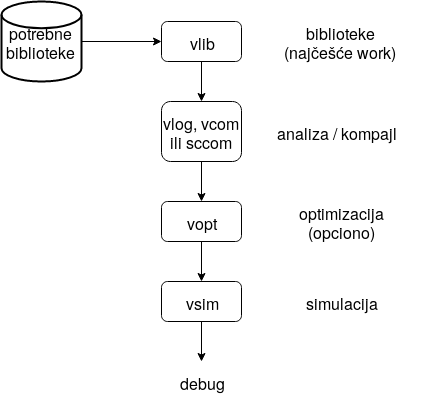
\includegraphics[width=90mm, scale=0.5]{img/v1_flow.png}
  \caption{QuestaSim flow}
  \label{fig:questa_flow}
\end{figure}

Za sve navedene korake postoje komande u Questasim-u (\emph{vlib, vlog, vsim,}
...).
Najčešće se komande grupišu u skriptu radi lakše upotrebe, ali je moguće unositi
ih direktno u terminal ili koristiti GUI.
U nastavku je dat opis komandi potrebnih za današnje vežbe.

%----------------------------------------------------------------------------------------

\subsection{Biblioteke}

Pre kompajliranja sors koda, mora se kreirati biblioteka u kojoj će se čuvati
svi kompajlirani fajlovi. Obično se biblioteka zove \emph{work} i ukoliko se
eksplicitno ne navede naziv podrazumeva se \emph{work}.

\begin{itemize}
\item GUI: File \(\rightarrow\) New \(\rightarrow\) Library
\item CLI: vlib \textless lib\(\_\)name\textgreater
\end{itemize}

%----------------------------------------------------------------------------------------

\subsection{Kompajliranje}

Za kompajliranje dizajna postoje različite komande na osnovu jezika u kome je
implementiran.

\begin{itemize}
\item GUI: Compile \(\rightarrow\) Compile
\item CLI: vlog (Verilog), vcom (VHDL), sscom (SystemC) praćeno listom fajlova
\end{itemize}

Za kompajliranje SystemVerilog fajlova se takođe koristi naredba \emph{vlog},
ali uz -sv argument. Npr.:

\begin{lstlisting}[language=Python]
vlog -sv counter.sv simple_tb.sv
\end{lstlisting}

Korisni argumenti su i -work \textless ime\(\_\)biblioteke\textgreater kako bi
se rezultati smeštali u željenu biblioteku, +incdir+\textless
ime\(\_\)direktorijuma\textgreater za uključivanje dodatnog foldera i +acc kako
bi se omogućio pristup svim signalima u dizajnu.\\

Prilikom kompajliranja QuestaSim vrši ispis svih kompajliranih modula, ali i
navodi ime top modula.
Taj top modul ćemo koristiti za simulaciju u narednom koraku.
Na primer:

\begin{verbatim}
# QuestaSim vlog ...
# -- Compiling module counter
# -- Compiling module simple_tb
#
# Top level modules:
#        simple_tb
\end{verbatim}

%----------------------------------------------------------------------------------------

\subsection{Simulacija}

Učitavanje u simulator:
\begin{itemize}
\item GUI: Simulate \(\rightarrow\) Start simulation
\item CLI: vsim \textless top\(\_\)name\textgreater
\end{itemize}

Simulatoru se prosleđuje ime top modula koji želimo da simuliramo.\\

Kada se dizajn učita u simulator, simulaciono vreme je nula i čeka se na dalje
komande za pokretanje simulacije.
Ovo se vrši naredbom \emph{run}.
Moguće je pustiti simulaciju do kraja ili na određeni vremenski period.

\begin{lstlisting}[language=Python]
run -all
run 10us
\end{lstlisting}

%----------------------------------------------------------------------------------------

\subsection{Naredba do}

Korisna naredba u QuestaSim-u je \emph{do} koja služi za izvršavanje naredbi iz
fajla.
Da bi se ubrzao proces kompilacije i simulacije, obično se ove komande grupišu u
skriptu koju je tada lako pozivati iz alata (komentari započinju simbolom
``\(\#\)'').
Za prethodni primer testbenča:

% Note: nije python, ali dobro oboji :)
\lstinputlisting[language=Python, caption=do fajl, label=lst:do_fajl]{code/v1_run.do}

Kako bi smo izvršili ove naredbe, potrebno je u Questi pozvati
\begin{lstlisting}[language=Python]
do <ime_fajla>
\end{lstlisting}

%----------------------------------------------------------------------------------------

\subsection{Debug}

QuestaSim pruža veliki broj alata za analizu i debug dizajna.
Oni uključuju gledanje \emph{waveform}-a, postavljanje \emph{breakpoint}-a,
analizu povezanosti, praćenje pokrivenosti, ...
Većina će biti pokazana u narednim vežbama, dok ćemo se ovde, zbog
jednostavnosti primera, zadržati na gledanju \emph{waveform}-a.\\

\emph{Waveform}-i se prikazuju u tzv. \emph{wave} prozoru koji se aktivira sa
naredbom:
\begin{itemize}
\item GUI: View \(\rightarrow\) Wave
\item CLI: view wave
\end{itemize}

Dodavanje signala se može izvršiti na nekoliko načina:
\begin{itemize}
\item iz glavnog prozora, desnim klikom na željeni objekat i odabrati Add
  \(\rightarrow\) To Wave \(\rightarrow\) .... Poslednji korak su opcije koje
  označavaju opseg signala koje želimo da dodamo
\item dodavanjem pojedinačnih signala iz \emph{Objects} prozora na isti način
\item \emph{drag and drop}
\item komandom ``add wave \textless putanja\textgreater'' (podržava
  \emph{wildcard} ``*'' za dodavanje više signala)
\end{itemize}

Nakon učitavanja željenih signala, iz \emph{toolbar}-a je lako puštati
simulaciju.
Simulacija se može puštati do kraja ili određeni vremenski period, može se
prekidati, nastavljati, restartovati itd. (slika \ref{fig:questa_toolbar_run}).\\

\begin{figure}[h!]
  \center
  
\includegraphics[width=60mm, scale=0.5]{img/v1_toolbar_run.png}
  \caption{QuestaSim run toolbar}
  \label{fig:questa_toolbar_run}
\end{figure}

Analizu signala olakšava zumiranje, praćenje ivica, praćenje kursora koji se
takođe lako kontorlišu iz \emph{toolbar}-a (slika
\ref{fig:questa_toolbar_zoom})\\

\begin{figure}[h!]
  \center
  
\includegraphics[width=60mm, scale=0.5]{img/v1_toolbar_zoom.png}
  \caption{QuestaSim zoom toolbar}
  \label{fig:questa_toolbar_zoom}
\end{figure}

Nakon ubacivanja signala u \emph{wave} prozor i svih dodatnih podešavanja,
moguće je sačuvati sva podešavanja u \emph{do} fajl.
Podrazumevano ime je ``wave.do'' i izvršava se kao i svi \emph{do} fajlovi:

\begin{lstlisting}[language=Python]
do wave.do 
\end{lstlisting}

QuestaSim pruža velike mogućnosti rada sa \emph{waveform}-ima, uključujući i
poređenje signala, čuvanje podešavanja za buduću upotrebu, merenje vremena, ...
Za detaljan opis svih mogućnosti konsultovati \emph{User Manual}, koji se može
naći u QuestaSim-u (Help \(\rightarrow\) Questa Documentation).

%========================================================================================
% Section
%========================================================================================

\section{Zadaci}

\paragraph{Zadatak}

Koristeći primer jednostavnog testbenča za brojač, pokrenuti simulaciju i
analizirati rezultate.
Uočiti razlike između \emph{initial}, \emph{always} i \emph{final} blokova.
Pogledati \emph{waveform}-e.
Pogledati kako menjanje \emph{timescale}-a utiče na simulaciju.

\paragraph{Zadatak}

Napisati blok za generisanje stimulusa odnosno generisanje signala
\emph{ce\(\_\)i} i \emph{up\(\_\)i}.

\paragraph{Zadatak}

Napisati monitor blok za proveru vrednosti brojača.
Vrednosti porediti funkcijom \emph{compare\(\_\)values}.

%========================================================================================

